\chapter{Experiments: Regular Tilings}

\textcolor{red}{
  \textbf{Methodology:} We look at the three most common types of tilings by
regular polygons: regular tilings. Grünbaum and Shephard (section 1.3) about
tilings, talks about regularity. ``Edge-to-edge'' tiling by congruent regular
polygons. The three regular tesselations, or Euclidean tilings, are square,
triangular, and hexagonal.
}

\textcolor{red}{
  There also exists semiregular, often called uniform, tilings, where there are
two or more faces. There are also more complex schemes, but we are interested in
tilings that are lattice-like. The different types of Bravais lattices for 2
dimensions were all investigated, but using just regular tilings was found to be
sufficient. We are not necessarily interesting in comparing lattice structures
directly, but rather in the applicability of such structures in general.
}

\textcolor{blue}{
  ``Lattice networks/models are common in computational physics, condensed
matter physics and beyond, modelling physical interactions, phase transitions
and structure [15]. Examples include: discrete lattices like the Ising model
with variables representing magnetic dipole moments of atomic spins, and the
Gray- Scott reaction-diffusion model to simulate chemical systems [22]. Also,
physical substrates often have a regular grid of connections. Lattice networks
are therefore more realistic representations of many physical systems that would
be considered for reservoir computing.'', Role of Structure and Complexity, Dale
et al.
}

% (TODO): t!
\begin{figure*}[t]
  \centering
  \begin{subfigure}{.32\textwidth}
    \centering
    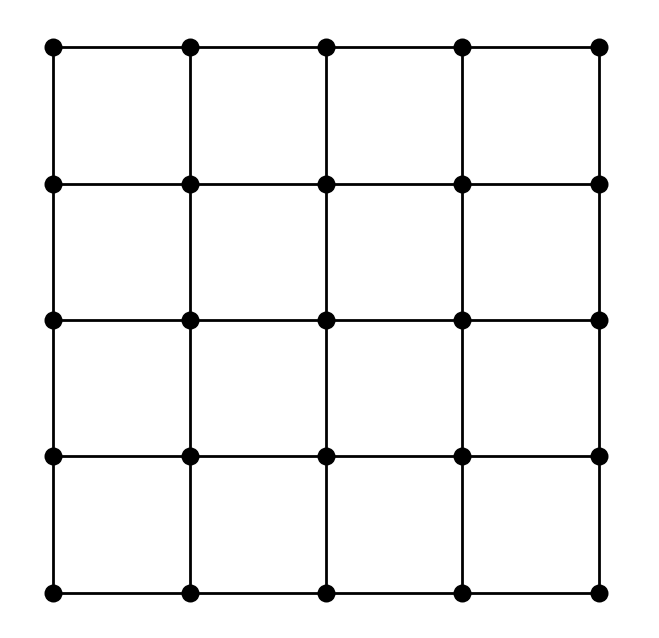
\includegraphics[width=1.0\linewidth]{figures/square.png}
    \label{fig:rt-square}
  \end{subfigure}
  \begin{subfigure}{.32\textwidth}
    \centering
    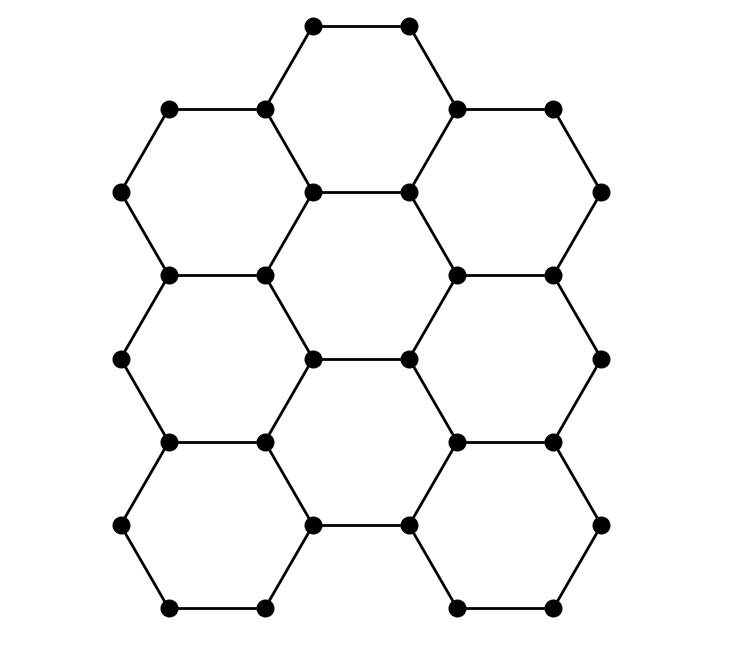
\includegraphics[width=1.0\linewidth]{figures/hex.png}
    \label{fig:rt-hex}
  \end{subfigure}
  \begin{subfigure}{.32\textwidth}
    \centering
    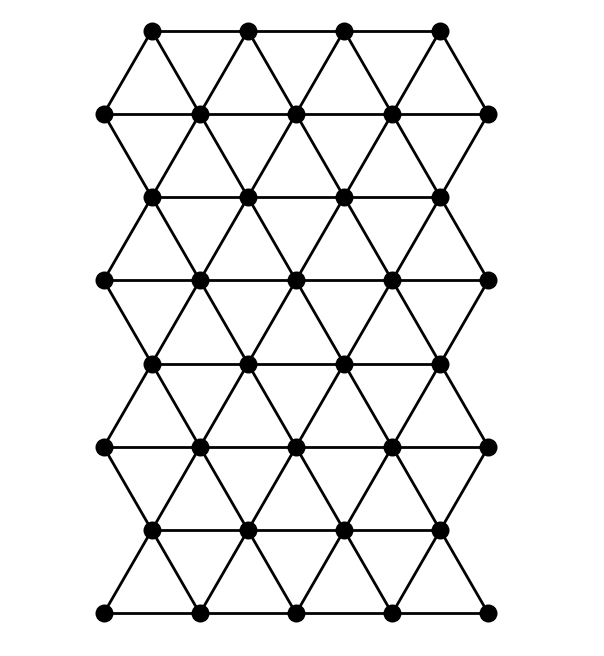
\includegraphics[width=1.0\linewidth]{figures/triangular.png}
    \label{fig:rt-tri}
  \end{subfigure}
  \caption{
    Regular tilings investigated for their quality as reservoir
topologies. Investigated topologies include square (a), hexagonal (b), and
triangular (c) regular tilings.
  }
  \label{fig:regular-tilings}
\end{figure*}

\section{Methodology}

% (TODO): Chapter reference.
\textcolor{red}{
  \textbf{Methodology:} We use the same base as provided by the chapter on
methodology, but replace the weight matrix of the reservoir, i.e. its innards,
with that of the lattice structures we generate. This provides connectivity
within the reservoir of regular, spatially constrained nature. Everything else
should be the same.
}

\section{Reservoir Quality of Regular Tilings}

\subsection{Synopsis}

\subsection{Results and Discussion}

\subsection{Summary}

\section{Regular Tilings with Directed Edges}

\subsection{Synopsis}

\subsection{Results and Discussion}

Should include both going to directed edges as well as changing to global input.

Should include an example of great performance vs. one of not so good
performance.

Should perhaps also talk about MC and KQ/G.

Also include harder NARMA orders at the end here when talking about this.

\subsection{Summary}

\section{Shrinking and Growing Directed Reservoirs}

\subsection{Synopsis}

\subsection{Results and Discussion}

Should include both shrinking and growing reservoirs for a conjoined discussion.

\subsection{Summary}

\section{Restoring Bidirectional Edges}

\subsection{Synopsis}

\subsection{Results and Discussion}

\subsection{Summary}

\section{Conclusion}


%%% Local Variables:
%%% mode: latex
%%% TeX-master: "../thesis"
%%% End:
